\documentclass{article}
\usepackage[%
    left=0.5in,%
    right=0.5in,%
    top=0.5in,%
    bottom=0.5in,%
]{geometry}%
\usepackage{minitoc}
\usepackage{multicol}
\usepackage{graphicx}
\usepackage{fixltx2e}
\usepackage{hyperref}
\usepackage{hyperref}
    \hypersetup{ colorlinks = true, linkcolor = blue }
\usepackage{blindtext}

\graphicspath{ {./} }

\newcommand{\inlinecode}[2]{\colorbox{lightgray}{\lstinline
[language=#1]$#2$}}
\newcommand{\worddef}[1]{\hyperref[sec:reference]{\textit{#1}}}

\begin{document}

\section{Simple Implementations of a Priority Queue}
\begin{itemize}
	\item Implementation with an unsorted list
	\begin{itemize}
		\item \texttt{insert(n)} is $O(1)$
		\item \texttt{min(n)} and \texttt{removeMin(n)} is $O(n)$ 
	\end{itemize}
	\item Implementation with an sorted list
	\begin{itemize}
		\item \texttt{insert(n)} is $O(n)$
		\item \texttt{min(n)} and \texttt{removeMin(n)} is $O(1)$ (always at head)
	\end{itemize}
\end{itemize}

\section{Binary heap}
\begin{flushleft}
A heap is a binary tree storing key-value pairs at its nodes and satisfying the following properties:
\begin{itemize}
	\item \textbf{Heap-Order}: for every internal node $v$ other than the \textbf{root}, $key(v) \geq key(parent(v))$
	\item \textbf{Complete Binary Tree}
	\begin{itemize}
		\item let $h$ be the height of the heap for $i = 0$, … , $h - 1$, there are $2^i$ nodes of depth i
		\item At depth $h - 1$, the nodes are to the \textbf{left} of any \textbf{missing nodes}
	\end{itemize}
\end{itemize}
\end{flushleft}

\subsection{Height}
\begin{flushleft}
\textbf{Theorem}: A heap storing $n$ keys has height $O(log \mathbf{n})$ Proof: This uses just the complete binary tree property
\end{flushleft}

\subsection{Insertion into a Heap}
\begin{flushleft}
Method \texttt{insertItem} of the priority queue ADT corresponds to the insertion of a key $k$ to the heap. The insertion algorithm consists of three steps
\begin{itemize}
	\item Find the insertion node $z$ (the new last node)
	\item Store $k$ at $z$
	\item Restore the heap-order property (discussed next)
\end{itemize}
\end{flushleft}

\subsection{Unheap}
\begin{itemize}
	\item After the insertion of a new key $k$, the heap-order property may be violated
	\item Algorithm upheap restores the heap-order property by swapping $k$ along an \textbf{upward path} from the insertion node
	\item Upheap terminates when the key $k$ reaches the root or a node whose parent has a key \textbf{smaller than or equal} to $k$
	\item Since a heap has height $O(log n)$, upheap runs in $O(log n)$ time
\end{itemize}

\subsection{Removal from a Heap}
\begin{flushleft}
Method \texttt{removeMin} of the priority queue ADT corresponds to the removal of the \textbf{root} key from the heap. The removal algorithm consists of three steps:
\begin{itemize}
	\item Replace the root key with the key of the last node $w$
	\item Remove $w$
	\item Restore the heap-order property (discussed next)
\end{itemize}
\end{flushleft}
\begin{center}
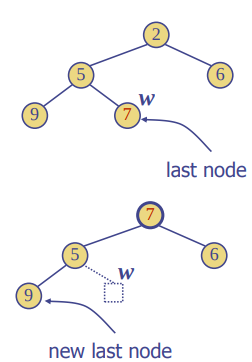
\includegraphics[scale=0.5]{heap_removeMin.png}
\end{center}

\subsection{Downheap}
\begin{flushleft}
After replacing the \textbf{root} key with the key $k$ of the \textbf{last} node, the \textit{heap-order property} may be violated. Algorithm \textit{downheap} restores the heap-order property by \textbf{swapping} key $k$ along a particular downward path from the root. Downheap terminates when key $k$ reaches a leaf or a node whose children have keys \textbf{greater than or equal} to $k$. Since a heap has height $O(log n)$, downheap runs in $O(log n)$ time
\end{flushleft}

\subsection{Array List Heap Implementation}
\begin{itemize}
	\item We can represent a heap with $n$ keys by means of a vector or ArrayList of length n + 1
	\item Links between nodes are not explicitly stored, instead:
	\item For the node at index $i$: 
	\begin{itemize}
		\item Left child is at index $2i$
		\item Right child is at index $2i + 1$
		\item Parent is at index $i/2$ 
	\end{itemize}
	\item The cell of at index $0$ is not used (Would mess up children indixes)
	\item Notice that there are \textbf{no gaps} when storing a heap
\end{itemize}
\begin{itemize}
	\item Operation \texttt{insert} corresponds to inserting at index $n + 1$
	\item Operation \texttt{removeMin} corresponds to moving index $n$ to index $1$
	\item Up- and down-heap operations just swap appropriate elements within the array
	\item Together with the \textbf{lack of gaps}, this makes the implementation very \textbf{efficient}, and this is the standard way to implement a Heap.
\end{itemize}

\end{document}
